% Options for packages loaded elsewhere
\PassOptionsToPackage{unicode}{hyperref}
\PassOptionsToPackage{hyphens}{url}
\PassOptionsToPackage{dvipsnames,svgnames,x11names}{xcolor}
%
\documentclass[
  letterpaper,
  DIV=11,
  numbers=noendperiod]{scrartcl}

\usepackage{amsmath,amssymb}
\usepackage{iftex}
\ifPDFTeX
  \usepackage[T1]{fontenc}
  \usepackage[utf8]{inputenc}
  \usepackage{textcomp} % provide euro and other symbols
\else % if luatex or xetex
  \usepackage{unicode-math}
  \defaultfontfeatures{Scale=MatchLowercase}
  \defaultfontfeatures[\rmfamily]{Ligatures=TeX,Scale=1}
\fi
\usepackage{lmodern}
\ifPDFTeX\else  
    % xetex/luatex font selection
\fi
% Use upquote if available, for straight quotes in verbatim environments
\IfFileExists{upquote.sty}{\usepackage{upquote}}{}
\IfFileExists{microtype.sty}{% use microtype if available
  \usepackage[]{microtype}
  \UseMicrotypeSet[protrusion]{basicmath} % disable protrusion for tt fonts
}{}
\makeatletter
\@ifundefined{KOMAClassName}{% if non-KOMA class
  \IfFileExists{parskip.sty}{%
    \usepackage{parskip}
  }{% else
    \setlength{\parindent}{0pt}
    \setlength{\parskip}{6pt plus 2pt minus 1pt}}
}{% if KOMA class
  \KOMAoptions{parskip=half}}
\makeatother
\usepackage{xcolor}
\setlength{\emergencystretch}{3em} % prevent overfull lines
\setcounter{secnumdepth}{-\maxdimen} % remove section numbering
% Make \paragraph and \subparagraph free-standing
\ifx\paragraph\undefined\else
  \let\oldparagraph\paragraph
  \renewcommand{\paragraph}[1]{\oldparagraph{#1}\mbox{}}
\fi
\ifx\subparagraph\undefined\else
  \let\oldsubparagraph\subparagraph
  \renewcommand{\subparagraph}[1]{\oldsubparagraph{#1}\mbox{}}
\fi

\usepackage{color}
\usepackage{fancyvrb}
\newcommand{\VerbBar}{|}
\newcommand{\VERB}{\Verb[commandchars=\\\{\}]}
\DefineVerbatimEnvironment{Highlighting}{Verbatim}{commandchars=\\\{\}}
% Add ',fontsize=\small' for more characters per line
\usepackage{framed}
\definecolor{shadecolor}{RGB}{241,243,245}
\newenvironment{Shaded}{\begin{snugshade}}{\end{snugshade}}
\newcommand{\AlertTok}[1]{\textcolor[rgb]{0.68,0.00,0.00}{#1}}
\newcommand{\AnnotationTok}[1]{\textcolor[rgb]{0.37,0.37,0.37}{#1}}
\newcommand{\AttributeTok}[1]{\textcolor[rgb]{0.40,0.45,0.13}{#1}}
\newcommand{\BaseNTok}[1]{\textcolor[rgb]{0.68,0.00,0.00}{#1}}
\newcommand{\BuiltInTok}[1]{\textcolor[rgb]{0.00,0.23,0.31}{#1}}
\newcommand{\CharTok}[1]{\textcolor[rgb]{0.13,0.47,0.30}{#1}}
\newcommand{\CommentTok}[1]{\textcolor[rgb]{0.37,0.37,0.37}{#1}}
\newcommand{\CommentVarTok}[1]{\textcolor[rgb]{0.37,0.37,0.37}{\textit{#1}}}
\newcommand{\ConstantTok}[1]{\textcolor[rgb]{0.56,0.35,0.01}{#1}}
\newcommand{\ControlFlowTok}[1]{\textcolor[rgb]{0.00,0.23,0.31}{#1}}
\newcommand{\DataTypeTok}[1]{\textcolor[rgb]{0.68,0.00,0.00}{#1}}
\newcommand{\DecValTok}[1]{\textcolor[rgb]{0.68,0.00,0.00}{#1}}
\newcommand{\DocumentationTok}[1]{\textcolor[rgb]{0.37,0.37,0.37}{\textit{#1}}}
\newcommand{\ErrorTok}[1]{\textcolor[rgb]{0.68,0.00,0.00}{#1}}
\newcommand{\ExtensionTok}[1]{\textcolor[rgb]{0.00,0.23,0.31}{#1}}
\newcommand{\FloatTok}[1]{\textcolor[rgb]{0.68,0.00,0.00}{#1}}
\newcommand{\FunctionTok}[1]{\textcolor[rgb]{0.28,0.35,0.67}{#1}}
\newcommand{\ImportTok}[1]{\textcolor[rgb]{0.00,0.46,0.62}{#1}}
\newcommand{\InformationTok}[1]{\textcolor[rgb]{0.37,0.37,0.37}{#1}}
\newcommand{\KeywordTok}[1]{\textcolor[rgb]{0.00,0.23,0.31}{#1}}
\newcommand{\NormalTok}[1]{\textcolor[rgb]{0.00,0.23,0.31}{#1}}
\newcommand{\OperatorTok}[1]{\textcolor[rgb]{0.37,0.37,0.37}{#1}}
\newcommand{\OtherTok}[1]{\textcolor[rgb]{0.00,0.23,0.31}{#1}}
\newcommand{\PreprocessorTok}[1]{\textcolor[rgb]{0.68,0.00,0.00}{#1}}
\newcommand{\RegionMarkerTok}[1]{\textcolor[rgb]{0.00,0.23,0.31}{#1}}
\newcommand{\SpecialCharTok}[1]{\textcolor[rgb]{0.37,0.37,0.37}{#1}}
\newcommand{\SpecialStringTok}[1]{\textcolor[rgb]{0.13,0.47,0.30}{#1}}
\newcommand{\StringTok}[1]{\textcolor[rgb]{0.13,0.47,0.30}{#1}}
\newcommand{\VariableTok}[1]{\textcolor[rgb]{0.07,0.07,0.07}{#1}}
\newcommand{\VerbatimStringTok}[1]{\textcolor[rgb]{0.13,0.47,0.30}{#1}}
\newcommand{\WarningTok}[1]{\textcolor[rgb]{0.37,0.37,0.37}{\textit{#1}}}

\providecommand{\tightlist}{%
  \setlength{\itemsep}{0pt}\setlength{\parskip}{0pt}}\usepackage{longtable,booktabs,array}
\usepackage{calc} % for calculating minipage widths
% Correct order of tables after \paragraph or \subparagraph
\usepackage{etoolbox}
\makeatletter
\patchcmd\longtable{\par}{\if@noskipsec\mbox{}\fi\par}{}{}
\makeatother
% Allow footnotes in longtable head/foot
\IfFileExists{footnotehyper.sty}{\usepackage{footnotehyper}}{\usepackage{footnote}}
\makesavenoteenv{longtable}
\usepackage{graphicx}
\makeatletter
\def\maxwidth{\ifdim\Gin@nat@width>\linewidth\linewidth\else\Gin@nat@width\fi}
\def\maxheight{\ifdim\Gin@nat@height>\textheight\textheight\else\Gin@nat@height\fi}
\makeatother
% Scale images if necessary, so that they will not overflow the page
% margins by default, and it is still possible to overwrite the defaults
% using explicit options in \includegraphics[width, height, ...]{}
\setkeys{Gin}{width=\maxwidth,height=\maxheight,keepaspectratio}
% Set default figure placement to htbp
\makeatletter
\def\fps@figure{htbp}
\makeatother

\usepackage{booktabs}
\usepackage{caption}
\usepackage{longtable}
\usepackage{colortbl}
\usepackage{array}
\usepackage{anyfontsize}
\usepackage{multirow}
\KOMAoption{captions}{tableheading}
\makeatletter
\@ifpackageloaded{tcolorbox}{}{\usepackage[skins,breakable]{tcolorbox}}
\@ifpackageloaded{fontawesome5}{}{\usepackage{fontawesome5}}
\definecolor{quarto-callout-color}{HTML}{909090}
\definecolor{quarto-callout-note-color}{HTML}{0758E5}
\definecolor{quarto-callout-important-color}{HTML}{CC1914}
\definecolor{quarto-callout-warning-color}{HTML}{EB9113}
\definecolor{quarto-callout-tip-color}{HTML}{00A047}
\definecolor{quarto-callout-caution-color}{HTML}{FC5300}
\definecolor{quarto-callout-color-frame}{HTML}{acacac}
\definecolor{quarto-callout-note-color-frame}{HTML}{4582ec}
\definecolor{quarto-callout-important-color-frame}{HTML}{d9534f}
\definecolor{quarto-callout-warning-color-frame}{HTML}{f0ad4e}
\definecolor{quarto-callout-tip-color-frame}{HTML}{02b875}
\definecolor{quarto-callout-caution-color-frame}{HTML}{fd7e14}
\makeatother
\makeatletter
\makeatother
\makeatletter
\makeatother
\makeatletter
\@ifpackageloaded{caption}{}{\usepackage{caption}}
\AtBeginDocument{%
\ifdefined\contentsname
  \renewcommand*\contentsname{Table of contents}
\else
  \newcommand\contentsname{Table of contents}
\fi
\ifdefined\listfigurename
  \renewcommand*\listfigurename{List of Figures}
\else
  \newcommand\listfigurename{List of Figures}
\fi
\ifdefined\listtablename
  \renewcommand*\listtablename{List of Tables}
\else
  \newcommand\listtablename{List of Tables}
\fi
\ifdefined\figurename
  \renewcommand*\figurename{Figure}
\else
  \newcommand\figurename{Figure}
\fi
\ifdefined\tablename
  \renewcommand*\tablename{Table}
\else
  \newcommand\tablename{Table}
\fi
}
\@ifpackageloaded{float}{}{\usepackage{float}}
\floatstyle{ruled}
\@ifundefined{c@chapter}{\newfloat{codelisting}{h}{lop}}{\newfloat{codelisting}{h}{lop}[chapter]}
\floatname{codelisting}{Listing}
\newcommand*\listoflistings{\listof{codelisting}{List of Listings}}
\makeatother
\makeatletter
\@ifpackageloaded{caption}{}{\usepackage{caption}}
\@ifpackageloaded{subcaption}{}{\usepackage{subcaption}}
\makeatother
\makeatletter
\@ifpackageloaded{tcolorbox}{}{\usepackage[skins,breakable]{tcolorbox}}
\makeatother
\makeatletter
\@ifundefined{shadecolor}{\definecolor{shadecolor}{rgb}{.97, .97, .97}}
\makeatother
\makeatletter
\makeatother
\makeatletter
\makeatother
\ifLuaTeX
  \usepackage{selnolig}  % disable illegal ligatures
\fi
\IfFileExists{bookmark.sty}{\usepackage{bookmark}}{\usepackage{hyperref}}
\IfFileExists{xurl.sty}{\usepackage{xurl}}{} % add URL line breaks if available
\urlstyle{same} % disable monospaced font for URLs
\hypersetup{
  pdftitle={Lab 2},
  pdfauthor={Your Name Here},
  colorlinks=true,
  linkcolor={blue},
  filecolor={Maroon},
  citecolor={Blue},
  urlcolor={Blue},
  pdfcreator={LaTeX via pandoc}}

\title{Lab 2}
\usepackage{etoolbox}
\makeatletter
\providecommand{\subtitle}[1]{% add subtitle to \maketitle
  \apptocmd{\@title}{\par {\large #1 \par}}{}{}
}
\makeatother
\subtitle{BSTA 512/612}
\author{Your Name Here}
\date{}

\begin{document}
\maketitle
\ifdefined\Shaded\renewenvironment{Shaded}{\begin{tcolorbox}[interior hidden, borderline west={3pt}{0pt}{shadecolor}, enhanced, boxrule=0pt, breakable, frame hidden, sharp corners]}{\end{tcolorbox}}\fi

\begin{tcolorbox}[enhanced jigsaw, left=2mm, opacitybacktitle=0.6, arc=.35mm, colback=white, colframe=quarto-callout-caution-color-frame, bottomrule=.15mm, opacityback=0, toptitle=1mm, toprule=.15mm, titlerule=0mm, colbacktitle=quarto-callout-caution-color!10!white, rightrule=.15mm, leftrule=.75mm, title=\textcolor{quarto-callout-caution-color}{\faFire}\hspace{0.5em}{Caution}, breakable, bottomtitle=1mm, coltitle=black]

This lab is ready to go! Nicky (1/28/2025)

\end{tcolorbox}

\hypertarget{directions}{%
\subsection{Directions}\label{directions}}

Please turn in your \texttt{.html} file
\href{https://sakai.ohsu.edu/portal/site/BSTA-512-1-AC-W25/tool/af1e1389-d708-4fe2-94b3-caa1b503592b?panel=Main}{on
Sakai.} Please let me know if you greatly prefer to submit a physical
copy.

\href{https://github.com/nwakim/BSTA_512_W25/blob/main/labs/Lab_02.qmd}{You
can download the \texttt{.qmd} file for this lab here.} Please use the
linked qmd file and not this one! (This is specifically the
instructions.)

The rest of this lab's instructions are embedded into the lab
activities.

\hypertarget{purpose}{%
\subsubsection{Purpose}\label{purpose}}

The main purpose of this lab is to introduce our dataset, codebook, and
variables. We will continue to think about the context of our research
question, but our main focus is to become familiar with the data.

\hypertarget{grading}{%
\subsubsection{Grading}\label{grading}}

\textbf{This lab is graded out of 12 points.} Nicky will use the
following rubric displayed on the \href{../project.qmd}{Project} page.

\hypertarget{lab-activities}{%
\subsection{Lab activities}\label{lab-activities}}

\hypertarget{access-and-download-the-data}{%
\subsubsection{1. Access and download the
data}\label{access-and-download-the-data}}

This serves as good practice for accessing data that is online or needs
to be downloaded from a collaborator.

Data can be accessed \href{https://osf.io/iay3x/}{here}. Under ``Weight
IAT 2004-2024'' there are several drop down menus:

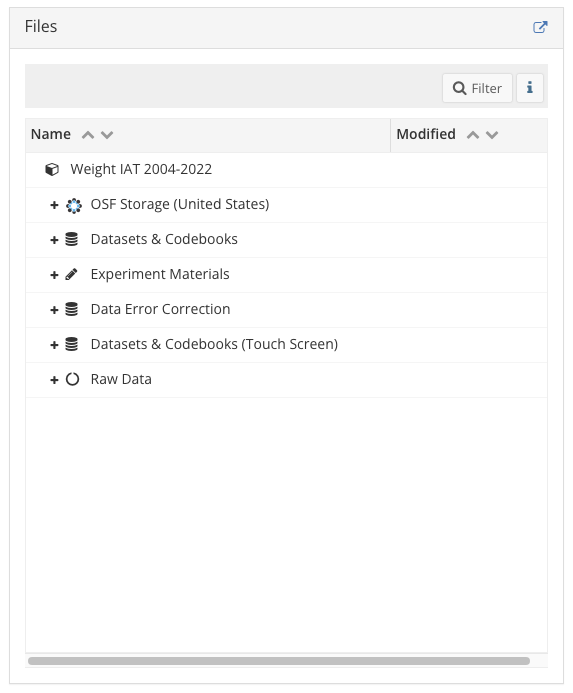
\includegraphics{images/data_access_1.png}

I opened the first ``Datasets \& Codebooks,'' then selected ``OSF
Storage (United States).'' Once selected, the ``Download as zip'' option
pops up in the top right part of the Files section.

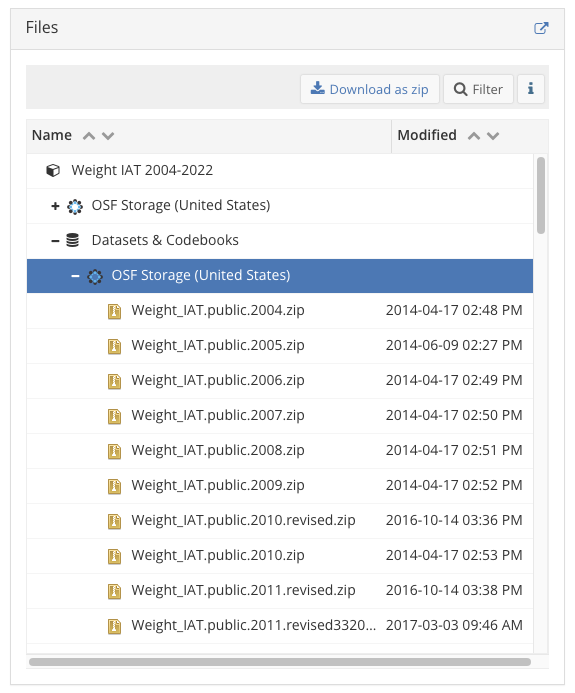
\includegraphics{images/data_access_2.png}

We will be working with the \texttt{Weight\_IAT.public.2021.csv}
dataset. Please locate the \texttt{zip} file called
\texttt{Weight\ IAT.public.2021-CSV.zip} . To download, you need to
click the row of the zip file, but you can't click the name of the zip
file. If a link opens, then you clicked the name. If the row is
highlighted blue and clickable ``Download'' and ``View'' buttons appear
on the top right, then you selected it correctly! (See below image for
what it should look like.)

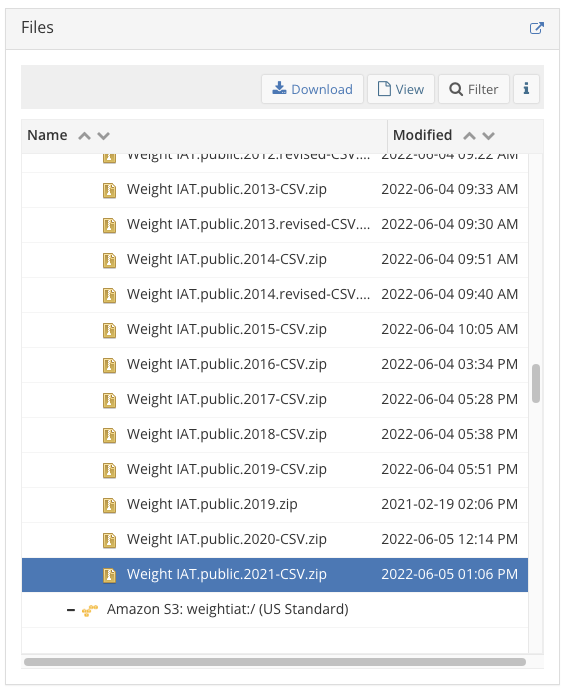
\includegraphics{images/data_access_3.png}

Then click the ``Download'' button to download! Note that the name does
not have an underscore between ``Weight'' and ``IAT.'' I like to have my
datasets named without spaces, so I will replace the space with an
underscore.

For the codebook, perform the same process for the file named:
\texttt{Weight\_IAT\_public\_2021\_codebook.xlsx}

You will need to unzip the actual data.

Move the data to a folder that you can easily access as you work from
this document. I like to have a folder named \texttt{data} to house my
data.

\begin{tcolorbox}[enhanced jigsaw, left=2mm, opacitybacktitle=0.6, arc=.35mm, colback=white, colframe=quarto-callout-important-color-frame, bottomrule=.15mm, opacityback=0, toptitle=1mm, toprule=.15mm, titlerule=0mm, colbacktitle=quarto-callout-important-color!10!white, rightrule=.15mm, leftrule=.75mm, title=\textcolor{quarto-callout-important-color}{\faExclamation}\hspace{0.5em}{Task Summary}, breakable, bottomtitle=1mm, coltitle=black]

Download the 2021 data and codebook from the archives and store in
accessible folder.

\end{tcolorbox}

\hypertarget{load-data-and-needed-packages}{%
\subsubsection{2. Load data and needed
packages}\label{load-data-and-needed-packages}}

First, load the packages that you will need in the remainder of this
lab. You can add to this as you need to. At the top of your R code
chunk, you can add the following option to repress the messages from the
loading packages:

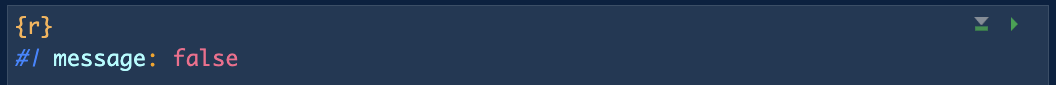
\includegraphics{images/r_message.png}

\begin{Shaded}
\begin{Highlighting}[]
\FunctionTok{library}\NormalTok{(tidyverse)}
\FunctionTok{library}\NormalTok{(gtsummary)}
\FunctionTok{library}\NormalTok{(here)}
\ControlFlowTok{if}\NormalTok{(}\SpecialCharTok{!}\FunctionTok{require}\NormalTok{(lubridate)) \{ }\FunctionTok{install.packages}\NormalTok{(}\StringTok{"lubridate"}\NormalTok{); }\FunctionTok{library}\NormalTok{(lubridate) \}}
\end{Highlighting}
\end{Shaded}

Using R, load the data (\texttt{csv} file) into this document. Note that
this is a \texttt{csv} file that we can load with basic R packages. Name
your dataset something that feels intuitive to you and will distinguish
it from other datasets that you work with.

Loading the \texttt{csv} file every time you render will take a long
time. One way to speed this up is by saving the data as an \texttt{rda}
file (R data file). Change the following R code to save the \texttt{rda}
file. You will also need to remove the
\texttt{\#\textbar{}\ eval:\ false} at the top of the code chunk once
you have corrected the code. If you are confused on the syntax, don't
forget that you can use \texttt{?save} for more information.

\begin{Shaded}
\begin{Highlighting}[]
\FunctionTok{save}\NormalTok{(}\SpecialCharTok{\textless{}}\NormalTok{whatever you called the read csv file}\SpecialCharTok{\textgreater{}}\NormalTok{, }\AttributeTok{file =} \StringTok{"Where you would like to save the file with its name"}\NormalTok{)}
\end{Highlighting}
\end{Shaded}

Check that you have an \texttt{rda} file where you saved it. Now use
\texttt{load()} with the file path to load the \texttt{rda} data here.

\begin{Shaded}
\begin{Highlighting}[]
\FunctionTok{load}\NormalTok{(}\AttributeTok{file =} \StringTok{"Where you would like to save the file with its name"}\NormalTok{)}
\end{Highlighting}
\end{Shaded}

At this point, if you think you loaded the file correctly, add
\texttt{\#\textbar{}\ eval:\ false} to the code chunk where you loaded
the \texttt{csv} file and back to the chunk where you saved the
\texttt{rda} file.

Take a \texttt{glimpse} at the data to make sure you loaded it
correctly.

How many rows and columns are in the dataset? Do you think we will need
all these variables for our analysis?

\begin{tcolorbox}[enhanced jigsaw, left=2mm, opacitybacktitle=0.6, arc=.35mm, colback=white, colframe=quarto-callout-important-color-frame, bottomrule=.15mm, opacityback=0, toptitle=1mm, toprule=.15mm, titlerule=0mm, colbacktitle=quarto-callout-important-color!10!white, rightrule=.15mm, leftrule=.75mm, title=\textcolor{quarto-callout-important-color}{\faExclamation}\hspace{0.5em}{Task Summary}, breakable, bottomtitle=1mm, coltitle=black]

Read csv, save as rda, load rda, glimpse at data.

How many rows and columns are in the dataset? Do you think we will need
all these variables for our analysis?

\end{tcolorbox}

\hypertarget{data-wrangling}{%
\subsubsection{3. Data wrangling}\label{data-wrangling}}

As you go through this process, it is important that you look at the
codebook for more information on each variable.

\hypertarget{whats-our-target-population}{%
\paragraph{3.1 What's our target
population?}\label{whats-our-target-population}}

As many of you mentioned in Lab 1, individuals taking the IAT test are
not necessarily representative of the world population. I want you to
articulate the target population that you think our analysis can give
information about. To what population can we generalize our analysis
results? We can get very specific with this population, but try to
restrict your population to 3-5 characteristics.

After you articulate the population, I want to add one more restriction
to our population: US residency. The sample includes individuals
residing in many different countries. Since we are discussing attitudes
and beliefs that is inherently connected to society and culture, I think
it is important that we restrict our analysis and discussion to a
country that we have some social experience in. \textbf{Thus, let's
restrict our data to the US only by filtering the variable
\texttt{countryres} to category 1 (corresponding to the US).}

\begin{tcolorbox}[enhanced jigsaw, left=2mm, opacitybacktitle=0.6, arc=.35mm, colback=white, colframe=quarto-callout-important-color-frame, bottomrule=.15mm, opacityback=0, toptitle=1mm, toprule=.15mm, titlerule=0mm, colbacktitle=quarto-callout-important-color!10!white, rightrule=.15mm, leftrule=.75mm, title=\textcolor{quarto-callout-important-color}{\faExclamation}\hspace{0.5em}{Task}, breakable, bottomtitle=1mm, coltitle=black]

Describe our target population. Keep your description to 3-5
characteristics, not including our restriction on the US population.

\end{tcolorbox}

\hypertarget{restrict-your-analysis-to-1-outcome-and-9-possible-covariatespredictors}{%
\paragraph{3.2 Restrict your analysis to 1 outcome and 9 possible
covariates/predictors}\label{restrict-your-analysis-to-1-outcome-and-9-possible-covariatespredictors}}

We are going to restrict our analysis to the single outcome, IAT score,
which is named \texttt{D\_biep.Thin\_Good\_all}. You can rename this
variable.

We will also restrict our analysis to the following 9 potential
variables so our work is a little more manageable.

\begin{tcolorbox}[enhanced jigsaw, left=2mm, opacitybacktitle=0.6, arc=.35mm, colback=white, colframe=quarto-callout-important-color-frame, bottomrule=.15mm, opacityback=0, toptitle=1mm, toprule=.15mm, titlerule=0mm, colbacktitle=quarto-callout-important-color!10!white, rightrule=.15mm, leftrule=.75mm, title=\textcolor{quarto-callout-important-color}{\faExclamation}\hspace{0.5em}{Task}, breakable, bottomtitle=1mm, coltitle=black]

From the following 8 attitudes and beliefs, please select 3 that you
think will be the most important variables related to your research
question. In 1-2 lines, briefly explain why you chose each variable.
This can be informal and bulleted.

\end{tcolorbox}

(Make sure you chose the variable that is part of your research
question!)

\begin{enumerate}
\def\labelenumi{\arabic{enumi}.}
\tightlist
\item
  Explicit anti-fat bias (\texttt{att7})
\item
  Self-perception of weight (\texttt{iam\_001})
\item
  Fat group identity (\texttt{identfat\_001} )
\item
  Thin group identity (\texttt{identthen\_001} )
\item
  Controllability of weight of others (\texttt{controlother\_001})
\item
  Controllability of weight of yourself (\texttt{controlyou\_001})
\item
  Awareness of societal standards (\texttt{mostpref\_001} )
\item
  Internalization of societal standards (\texttt{important\_001})
\end{enumerate}

We will start our data exploration with the following 4 demographic
variables:

\begin{enumerate}
\def\labelenumi{\arabic{enumi}.}
\tightlist
\item
  Age (we need to construct from \texttt{birthmonth},
  \texttt{birthyear}, \texttt{month}, and \texttt{year})
\item
  Race (\texttt{raceomb\_002} or \texttt{raceombmulti})
\item
  Ethnicity (\texttt{ethnicityomb})
\item
  Sex assigned at birth (\texttt{birthSex})
\end{enumerate}

Please pick 2 additional variables to include in your analysis:

\begin{enumerate}
\def\labelenumi{\arabic{enumi}.}
\tightlist
\item
  Education (\texttt{edu\_14})
\item
  Gender (\texttt{genderIdentity})
\item
  Self-reported BMI (through self-reported height and weight)
\item
  Political identity
\item
  Religion
\end{enumerate}

I have chosen these variables for a mixture of reasons. For example, I
have left out variables about residence and occupation because those
variables have hundreds of categories that would be overwhelming in
linear regression. For the 4 required demographic variables, I chose age
because I really want us to get practice with a continuous variable. I
chose race and ethnicity because of the intertwined history of racism
and anti-fat bias in Western countries (including the U.S. where most
participants reside).

\begin{tcolorbox}[enhanced jigsaw, left=2mm, opacitybacktitle=0.6, arc=.35mm, colback=white, colframe=quarto-callout-note-color-frame, bottomrule=.15mm, opacityback=0, toptitle=1mm, toprule=.15mm, titlerule=0mm, colbacktitle=quarto-callout-note-color!10!white, rightrule=.15mm, leftrule=.75mm, title=\textcolor{quarto-callout-note-color}{\faInfo}\hspace{0.5em}{A note of the available variables on race}, breakable, bottomtitle=1mm, coltitle=black]

The dataset has two separate race variables. One has mutually exclusive
categories (\texttt{raceomb\_002}) and the other allows participants to
make multiple selections (\texttt{raceombmulti}). The former
(\texttt{raceomb\_002}) allows one participant to identify with only one
race category.

\href{https://weallcount.com/2022/10/27/4-approaches-to-multiple-race-questions/}{Important
lesson from We All Count} about using a multiple selection race
question. We can try out all these options!

\end{tcolorbox}

Finally, I chose sex assigned at birth because adults in 2021 in the US
were likely raised in a society where your sex assigned at birth
impacted the gender stereotypes that you were raised in, which could
impact exposure to diet culture. This in addition to the many medical
conditions associated with one's sex assigned at birth that may affect
weight. The reason why I am leaving gender as an optional variable is
because the question on gender allows participants to chose multiple
options. The binary sex assigned at birth will make our analysis a
little easier from a statistics stand point. Unfortunately, we need to
balance achievable learning objectives and the most appropriate
variable. Since I have required race as a variable and has a multi-level
option, I do not want to overload our analysis with another multi-level
variable. Sex assigned at birth will not create more work for you (that
is outside of the course objectives) while capturing medical conditions
and \emph{some} of the societal impact of diet culture. This is
certainly a limitation in our analysis that we should address in our
discussion. I do encourage you to look into gender if the binary sex
assigned at birth does not feel right for you. I am happy to help!

\begin{tcolorbox}[enhanced jigsaw, left=2mm, opacitybacktitle=0.6, arc=.35mm, colback=white, colframe=quarto-callout-note-color-frame, bottomrule=.15mm, opacityback=0, toptitle=1mm, toprule=.15mm, titlerule=0mm, colbacktitle=quarto-callout-note-color!10!white, rightrule=.15mm, leftrule=.75mm, title=\textcolor{quarto-callout-note-color}{\faInfo}\hspace{0.5em}{A word on self-reported BMI}, breakable, bottomtitle=1mm, coltitle=black]

This variable is rooted in racism and anti-fat bias. The
\href{https://www.ama-assn.org/press-center/press-releases/ama-adopts-new-policy-clarifying-role-bmi-measure-medicine}{American
Medical Association made a few press releases} on policies using BMI as
a measure, with alternative measures (frankly, just other measures of
fatness to use as a diagnostic tool instead of checking true indicators
of health). However, I can think of a couple examples where BMI might
help us understand some context in this research, so I have left it as
an option. Although still self-reported, it might be interesting to see
how BMI (which is the closest measurement available in this dataset to
an ``objective'' measure of fatness) is related to individuals'
attitudes and beliefs. I am not saying there is anything to the
relationship, but it might be worth checking out if you are interested.

I will also say, in this dataset, there are MANY issues constructing the
variable for BMI from height and weight. \emph{If you do not feel
strongly about including it, I would suggest you avoid the variable
self-reported BMI}. It is not worth bringing in a racist and anti-fat
variable into the dataset if you do not have a specific use for it. If
you do plan to use it, please come to me for help as early as possible!

\end{tcolorbox}

If you would like to investigate a variable outside the list, please let
me know by emailing or chatting with me.

\begin{tcolorbox}[enhanced jigsaw, left=2mm, opacitybacktitle=0.6, arc=.35mm, colback=white, colframe=quarto-callout-important-color-frame, bottomrule=.15mm, opacityback=0, toptitle=1mm, toprule=.15mm, titlerule=0mm, colbacktitle=quarto-callout-important-color!10!white, rightrule=.15mm, leftrule=.75mm, title=\textcolor{quarto-callout-important-color}{\faExclamation}\hspace{0.5em}{Task}, breakable, bottomtitle=1mm, coltitle=black]

Using R, select your identified variables from your dataset.

\end{tcolorbox}

\hypertarget{manipulating-variables-that-are-coded-as-numeric-variables}{%
\paragraph{3.3 Manipulating variables that are coded as numeric
variables}\label{manipulating-variables-that-are-coded-as-numeric-variables}}

Many variables in this dataset are coded as numeric values, but have
specific categories linking up to the numbers. Using \texttt{mutate()}
and \texttt{cases()} similar to our Data Management lesson, please
create a new categorical variable with the specified categories from the
codebook. Make sure that you create a variable with a new name! Since
some of these variables are ordered categories, we will investigate if
it's appropriate to use the numeric or categorical version of the
variable.

\begin{tcolorbox}[enhanced jigsaw, left=2mm, opacitybacktitle=0.6, arc=.35mm, colback=white, colframe=quarto-callout-tip-color-frame, bottomrule=.15mm, opacityback=0, toptitle=1mm, toprule=.15mm, titlerule=0mm, colbacktitle=quarto-callout-tip-color!10!white, rightrule=.15mm, leftrule=.75mm, title=\textcolor{quarto-callout-tip-color}{\faLightbulb}\hspace{0.5em}{Example of how I would create new variable for self-perception of weight
(\texttt{iam\_001}):}, breakable, bottomtitle=1mm, coltitle=black]

By looking at the codebook, I see that respondents answer the following
question: ``Currently, I am:''

\begin{itemize}
\tightlist
\item
  ``Very underweight''
\item
  ``Moderately underweight''
\item
  ``Slightly underweight''
\item
  ``Neither underweight nor underweight''
\item
  ``Slightly overweight''
\item
  ``Moderately overweight''
\item
  ``Very overweight''
\end{itemize}

If I look at the data as is, I see that the variable is numeric.

\begin{Shaded}
\begin{Highlighting}[]
\NormalTok{iat\_2021 }\SpecialCharTok{\%\textgreater{}\%}
\NormalTok{  dplyr}\SpecialCharTok{::}\FunctionTok{select}\NormalTok{(iam\_001) }\SpecialCharTok{\%\textgreater{}\%}
  \FunctionTok{tbl\_summary}\NormalTok{()}
\end{Highlighting}
\end{Shaded}

\begin{table}
\fontsize{12.0pt}{14.4pt}\selectfont
\begin{tabular*}{\linewidth}{@{\extracolsep{\fill}}lc}
\toprule
\textbf{Characteristic} & \textbf{N = 465,886}\textsuperscript{\textit{1}} \\ 
\midrule\addlinespace[2.5pt]
iam\_001 &  \\ 
    1 & 2,023 (0.6\%) \\ 
    2 & 7,902 (2.4\%) \\ 
    3 & 24,399 (7.3\%) \\ 
    4 & 148,081 (44\%) \\ 
    5 & 88,566 (27\%) \\ 
    6 & 43,090 (13\%) \\ 
    7 & 18,978 (5.7\%) \\ 
    Unknown & 132,847 \\ 
\bottomrule
\end{tabular*}
\begin{minipage}{\linewidth}
\textsuperscript{\textit{1}}n (\%)\\
\end{minipage}
\end{table}

Again, I want to create a varaible with the answers instead of numbers,
so I will change transform the variable to include the text:

\begin{Shaded}
\begin{Highlighting}[]
\NormalTok{iat\_2021 }\OtherTok{=}\NormalTok{ iat\_2021 }\SpecialCharTok{\%\textgreater{}\%}
  \FunctionTok{mutate}\NormalTok{(}\AttributeTok{iam\_001\_f =} \FunctionTok{case\_match}\NormalTok{(iam\_001,}
                             \DecValTok{7} \SpecialCharTok{\textasciitilde{}} \StringTok{"Very overweight"}\NormalTok{,}
                             \DecValTok{6} \SpecialCharTok{\textasciitilde{}} \StringTok{"Moderately overweight"}\NormalTok{,}
                             \DecValTok{5} \SpecialCharTok{\textasciitilde{}} \StringTok{"Slightly overweight"}\NormalTok{,}
                             \DecValTok{4} \SpecialCharTok{\textasciitilde{}} \StringTok{"Neither underweight nor underweight"}\NormalTok{,}
                             \DecValTok{3} \SpecialCharTok{\textasciitilde{}} \StringTok{"Slightly underweight"}\NormalTok{,}
                             \DecValTok{2} \SpecialCharTok{\textasciitilde{}} \StringTok{"Moderately underweight"}\NormalTok{,}
                             \DecValTok{1} \SpecialCharTok{\textasciitilde{}} \StringTok{"Very underweight"}\NormalTok{,}
                             \AttributeTok{.default =} \ConstantTok{NA} \CommentTok{\# to add NA if unknown}
\NormalTok{                             ) }\SpecialCharTok{\%\textgreater{}\%} \FunctionTok{factor}\NormalTok{())}
\NormalTok{iat\_2021 }\SpecialCharTok{\%\textgreater{}\%}
\NormalTok{  dplyr}\SpecialCharTok{::}\FunctionTok{select}\NormalTok{(iam\_001\_f) }\SpecialCharTok{\%\textgreater{}\%}
  \FunctionTok{tbl\_summary}\NormalTok{()}
\end{Highlighting}
\end{Shaded}

\begin{table}
\fontsize{12.0pt}{14.4pt}\selectfont
\begin{tabular*}{\linewidth}{@{\extracolsep{\fill}}lc}
\toprule
\textbf{Characteristic} & \textbf{N = 465,886}\textsuperscript{\textit{1}} \\ 
\midrule\addlinespace[2.5pt]
iam\_001\_f &  \\ 
    Moderately overweight & 43,090 (13\%) \\ 
    Moderately underweight & 7,902 (2.4\%) \\ 
    Neither underweight nor underweight & 148,081 (44\%) \\ 
    Slightly overweight & 88,566 (27\%) \\ 
    Slightly underweight & 24,399 (7.3\%) \\ 
    Very overweight & 18,978 (5.7\%) \\ 
    Very underweight & 2,023 (0.6\%) \\ 
    Unknown & 132,847 \\ 
\bottomrule
\end{tabular*}
\begin{minipage}{\linewidth}
\textsuperscript{\textit{1}}n (\%)\\
\end{minipage}
\end{table}

\begin{Shaded}
\begin{Highlighting}[]
\FunctionTok{ggplot}\NormalTok{(}\AttributeTok{data=}\NormalTok{iat\_2021) }\SpecialCharTok{+}
  \FunctionTok{geom\_boxplot}\NormalTok{(}\FunctionTok{aes}\NormalTok{(}\AttributeTok{x =}\NormalTok{ iam\_001\_f, }\AttributeTok{y =}\NormalTok{ IAT\_score))}
\end{Highlighting}
\end{Shaded}

\begin{verbatim}
Warning: Removed 129215 rows containing non-finite outside the scale range
(`stat_boxplot()`).
\end{verbatim}

\begin{figure}[H]

{\centering 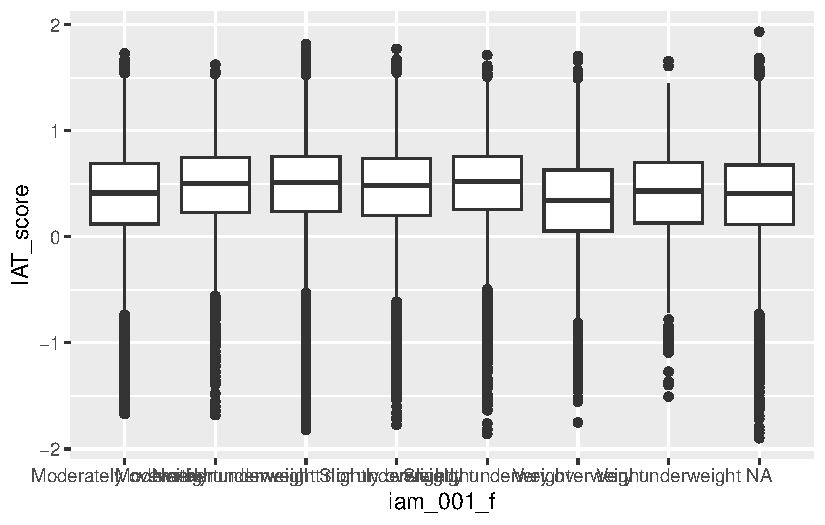
\includegraphics{Lab_02_instructions_files/figure-pdf/unnamed-chunk-7-1.pdf}

}

\end{figure}

I have called the new variable \texttt{iam\_001\_f} to indicate that the
variable is not in factor form. You can also call it something like
\texttt{iam\_001\_cat} to indicate the categorical form.

\end{tcolorbox}

\begin{tcolorbox}[enhanced jigsaw, left=2mm, opacitybacktitle=0.6, arc=.35mm, colback=white, colframe=quarto-callout-important-color-frame, bottomrule=.15mm, opacityback=0, toptitle=1mm, toprule=.15mm, titlerule=0mm, colbacktitle=quarto-callout-important-color!10!white, rightrule=.15mm, leftrule=.75mm, title=\textcolor{quarto-callout-important-color}{\faExclamation}\hspace{0.5em}{Task}, breakable, bottomtitle=1mm, coltitle=black]

Identify and list the variables that are coded numerically and
correspond to categories. Create a new variable for the
categorical/factor version of the variable. It is up to you to check
that your code ran properly!! If you are using multi-choice categorical
variables (might include race, gender), then do not convert the variable
yet!

\end{tcolorbox}

\hypertarget{creating-age-from-birth-date-and-test-date}{%
\paragraph{3.4 Creating age from birth date and test
date}\label{creating-age-from-birth-date-and-test-date}}

This dataset does not have an available ``age'' variable. However, we
have enough information to determine each individual's age from the test
date and their self-reported birth date. We can use the
\texttt{lubridate} package to configure the age. First, we need to use
\texttt{make\_date()} to construct the birth date and test date. Below,
I have implemented \texttt{make\_date()} to make the birth date.

\begin{tcolorbox}[enhanced jigsaw, left=2mm, opacitybacktitle=0.6, arc=.35mm, colback=white, colframe=quarto-callout-important-color-frame, bottomrule=.15mm, opacityback=0, toptitle=1mm, toprule=.15mm, titlerule=0mm, colbacktitle=quarto-callout-important-color!10!white, rightrule=.15mm, leftrule=.75mm, title=\textcolor{quarto-callout-important-color}{\faExclamation}\hspace{0.5em}{Task}, breakable, bottomtitle=1mm, coltitle=black]

From the codebook, find the variables that we can use to construct the
test date. Then use \texttt{make\_date()} to create the test date.

\end{tcolorbox}

\begin{Shaded}
\begin{Highlighting}[]
\NormalTok{iat\_2021 }\OtherTok{=}\NormalTok{ iat\_2021 }\SpecialCharTok{\%\textgreater{}\%}
  \FunctionTok{mutate}\NormalTok{(}\AttributeTok{birthdate =} \FunctionTok{make\_date}\NormalTok{(}\AttributeTok{month =}\NormalTok{ birthmonth, }\AttributeTok{year =}\NormalTok{ birthyear), }
         \AttributeTok{testdate =} \FunctionTok{make\_date}\NormalTok{(}\AttributeTok{month =}\NormalTok{ month, }\AttributeTok{year =}\NormalTok{ year))}
\end{Highlighting}
\end{Shaded}

Once the two dates are created, we can use further use
\texttt{lubridate} to calculate the age in years. This code is a little
complicated, so here is an example of how I have created age:

\begin{Shaded}
\begin{Highlighting}[]
\NormalTok{iat\_2021 }\OtherTok{=}\NormalTok{ iat\_2021 }\SpecialCharTok{\%\textgreater{}\%}
  \FunctionTok{mutate}\NormalTok{(}\AttributeTok{age =} \FunctionTok{interval}\NormalTok{(}\AttributeTok{start =}\NormalTok{ birthdate, }\AttributeTok{end =}\NormalTok{ testdate) }\SpecialCharTok{\%\textgreater{}\%}
          \FunctionTok{as.period}\NormalTok{() }\SpecialCharTok{\%\textgreater{}\%} \FunctionTok{year}\NormalTok{()) }\SpecialCharTok{\%\textgreater{}\%}
  \FunctionTok{select}\NormalTok{(}\SpecialCharTok{{-}}\NormalTok{birthmonth, }\SpecialCharTok{{-}}\NormalTok{birthyear, }\SpecialCharTok{{-}}\NormalTok{year, }\SpecialCharTok{{-}}\NormalTok{month, }
         \SpecialCharTok{{-}}\NormalTok{testdate, }\SpecialCharTok{{-}}\NormalTok{birthdate)}
\end{Highlighting}
\end{Shaded}

Note that the name of my dataset is \texttt{iat\_2021} and I feed it
into \texttt{mutate()}. Within \texttt{mutate()}, I assigned
\texttt{age} to the interval between the name of my birth date
(\texttt{birthdate}) and the name of my test date (\texttt{testdate}). I
need to convert the interval to a period of time (\texttt{as.period()}),
then to a measurement of years (\texttt{year()}).

\begin{tcolorbox}[enhanced jigsaw, left=2mm, opacitybacktitle=0.6, arc=.35mm, colback=white, colframe=quarto-callout-important-color-frame, bottomrule=.15mm, opacityback=0, toptitle=1mm, toprule=.15mm, titlerule=0mm, colbacktitle=quarto-callout-important-color!10!white, rightrule=.15mm, leftrule=.75mm, title=\textcolor{quarto-callout-important-color}{\faExclamation}\hspace{0.5em}{Task}, breakable, bottomtitle=1mm, coltitle=black]

Following the above example, create an age variable that measures the
years between individuals' birth and test date. Then remove the
variables used to make age.

\end{tcolorbox}

\hypertarget{if-you-chose-bmi-create-the-variable}{%
\paragraph{3.5 If you chose BMI, create the
variable}\label{if-you-chose-bmi-create-the-variable}}

Raw data from weight and height are categorical. This is according to
the codebook associated with this dataset. Please find your codebook
file named \texttt{Weight\_IAT\_public\_2021\_codebook.csv} . You can
find the value names for \texttt{myweight\_002} and
\texttt{myheight\_002}.

\begin{itemize}
\item
  For example, in the weight variable,

  \begin{itemize}
  \item
    most categories identify a lower limit to the weight in the group.
    One example group is weight is greater than or equal to 200 pounds
    and less than 205 pounds (labelled as ``200 lb :: 91 kg'').
  \item
    the first category for weight is ``below 50lb:: 23kg'' with 258
    observations
  \item
    the last category for weight is ``above 440lb:: above 200kg'' with
    295 observations

    \begin{itemize}
    \tightlist
    \item
      While the 5 groups of weight leading up the last category have 33,
      28, 34, 20, and 89 observations, respectively.
    \end{itemize}
  \end{itemize}
\end{itemize}

I will post an extra resource outlining some of my work on the BMI
variable.

\hypertarget{make-a-new-dataset-with-only-complete-cases}{%
\paragraph{3.6 Make a new dataset with only complete
cases}\label{make-a-new-dataset-with-only-complete-cases}}

Handling missing data is outside the scope of our class. There are many
techniques to handling missing data, but we will use complete case
analysis. This means we will only use observations that have information
for every variable we chose. The function \texttt{drop\_na()} will give
you the complete cases. You can feed your dataset into the function and
assign it as a new dataframe.

For example:

\begin{Shaded}
\begin{Highlighting}[]
\NormalTok{new\_df }\OtherTok{=}\NormalTok{ old\_df }\SpecialCharTok{\%\textgreater{}\%} \FunctionTok{drop\_na}\NormalTok{()}
\end{Highlighting}
\end{Shaded}

You will also need to save the new dataset so that you can load it in
future labs/work.

You can use something like:

\begin{Shaded}
\begin{Highlighting}[]
\FunctionTok{save}\NormalTok{(new\_df, }\AttributeTok{file =} \StringTok{"IAT\_data\_complete.Rda"}\NormalTok{)}
\end{Highlighting}
\end{Shaded}

Make sure this dataset saves into your project folder!

\begin{tcolorbox}[enhanced jigsaw, left=2mm, opacitybacktitle=0.6, arc=.35mm, colback=white, colframe=quarto-callout-important-color-frame, bottomrule=.15mm, opacityback=0, toptitle=1mm, toprule=.15mm, titlerule=0mm, colbacktitle=quarto-callout-important-color!10!white, rightrule=.15mm, leftrule=.75mm, title=\textcolor{quarto-callout-important-color}{\faExclamation}\hspace{0.5em}{Task}, breakable, bottomtitle=1mm, coltitle=black]

Make a new dataset with only complete cases. Save this dataset in your
project folder.

\end{tcolorbox}

\hypertarget{some-exploratory-data-analysis}{%
\subsubsection{4. Some exploratory data
analysis}\label{some-exploratory-data-analysis}}

\hypertarget{peek-at-your-outcome}{%
\paragraph{4.1 Peek at your outcome}\label{peek-at-your-outcome}}

This serves as a check to make sure we are all looking at the correct
outcome: IAT score.

\begin{tcolorbox}[enhanced jigsaw, left=2mm, opacitybacktitle=0.6, arc=.35mm, colback=white, colframe=quarto-callout-important-color-frame, bottomrule=.15mm, opacityback=0, toptitle=1mm, toprule=.15mm, titlerule=0mm, colbacktitle=quarto-callout-important-color!10!white, rightrule=.15mm, leftrule=.75mm, title=\textcolor{quarto-callout-important-color}{\faExclamation}\hspace{0.5em}{Task}, breakable, bottomtitle=1mm, coltitle=black]

Please plot a histogram of the IAT scores. What do you notice about the
outcome?

\end{tcolorbox}

\hypertarget{univariate-exploratory-data-analysis}{%
\paragraph{4.2 Univariate exploratory data
analysis}\label{univariate-exploratory-data-analysis}}

\begin{tcolorbox}[enhanced jigsaw, left=2mm, opacitybacktitle=0.6, arc=.35mm, colback=white, colframe=quarto-callout-important-color-frame, bottomrule=.15mm, opacityback=0, toptitle=1mm, toprule=.15mm, titlerule=0mm, colbacktitle=quarto-callout-important-color!10!white, rightrule=.15mm, leftrule=.75mm, title=\textcolor{quarto-callout-important-color}{\faExclamation}\hspace{0.5em}{Task}, breakable, bottomtitle=1mm, coltitle=black]

Using \texttt{ggplot} or tables, visualize your variables. Get a sense
of each variable's distribution. Do you notice anything out of the
ordinary?

\end{tcolorbox}

\hypertarget{bivariate-exploratory-data-analysis}{%
\paragraph{4.3 Bivariate exploratory data
analysis}\label{bivariate-exploratory-data-analysis}}

\begin{tcolorbox}[enhanced jigsaw, left=2mm, opacitybacktitle=0.6, arc=.35mm, colback=white, colframe=quarto-callout-important-color-frame, bottomrule=.15mm, opacityback=0, toptitle=1mm, toprule=.15mm, titlerule=0mm, colbacktitle=quarto-callout-important-color!10!white, rightrule=.15mm, leftrule=.75mm, title=\textcolor{quarto-callout-important-color}{\faExclamation}\hspace{0.5em}{Task}, breakable, bottomtitle=1mm, coltitle=black]

Take a look at the scatterplot, violin, or box plot of IAT score and
your variable of interest. Use R and \texttt{ggplot} to make this plot.
If your variable of interest is categorical, then make sure to use a
violin or boxplot.

\end{tcolorbox}

\hypertarget{revisit-your-research-question}{%
\subsubsection{5. Revisit your research
question}\label{revisit-your-research-question}}

\begin{tcolorbox}[enhanced jigsaw, left=2mm, opacitybacktitle=0.6, arc=.35mm, colback=white, colframe=quarto-callout-important-color-frame, bottomrule=.15mm, opacityback=0, toptitle=1mm, toprule=.15mm, titlerule=0mm, colbacktitle=quarto-callout-important-color!10!white, rightrule=.15mm, leftrule=.75mm, title=\textcolor{quarto-callout-important-color}{\faExclamation}\hspace{0.5em}{Task}, breakable, bottomtitle=1mm, coltitle=black]

Please restate the research question that you proposed in Lab 1. Please
make sure it is only one question, one sentence long. What are your
thoughts on the research question now that we looked at the data? Feel
free to change it now that we've looked at the data. If you change your
question, make sure 4.2 reflects the new research question.

\end{tcolorbox}

\begin{tcolorbox}[enhanced jigsaw, left=2mm, opacitybacktitle=0.6, arc=.35mm, colback=white, colframe=quarto-callout-note-color-frame, bottomrule=.15mm, opacityback=0, toptitle=1mm, toprule=.15mm, titlerule=0mm, colbacktitle=quarto-callout-note-color!10!white, rightrule=.15mm, leftrule=.75mm, title=\textcolor{quarto-callout-note-color}{\faInfo}\hspace{0.5em}{Note}, breakable, bottomtitle=1mm, coltitle=black]

In research, we typically do NOT change our research question after
looking at the data! Researchers typically form their questions from
other research and their expertise. We may not have expertise in this
field and we have not been studying implicit bias, so I want to be a
little more flexible with our analysis.

\end{tcolorbox}



\end{document}
